\chapter{Experiments and Results}
\label{chapter:experiments}

So far we have discussed the CCD approach in detail. In this chapter,
the experimental evaluation of the CCD algorithm and the naive CCD
tracker will be presented. We apply the CCD approach to three
different kinds of model fitting and object tracking problems:

\begin{enumerate}
\item Contour convergence on still image.
\item Tracking initiated from SIFT features.
\item Tracking initiated through back-projections of point clouds.
\end{enumerate}

Experiments have been carried out on the PR2 robot, we analyze the performance
of the approach in terms of robustness, accuracy and runtime. In the
end of the section, the comparison between the CCD approach and  other
model-based methods is given.


% by the experimental evaluation of the CCD
% algorithm. presents the evaluation of the naive CCD
% tracker and 

\section{Contour Convergence On Still Image}
\label{sec:ES}

% As mentioned in related work, the CCD algorithm is an effective
% segmentation method like other model-based segmentation algorithms.

A segmentation of an image $I: \Omega \subset R^2 \longrightarrow R$
is the partitioning of its domain into homogeneous regions
$\Omega_1,\ldots, \Omega_n \subset \Omega$. In a complex environment,
due to the texture, shading, poor contrast and clutter, a segmentation is
always a challenging problem % in (Fig.~\ref{fig:flower_m}).

% \begin{figure}[htbp]
%   \begin{minipage}[t]{0.5\linewidth} 
%     \centering 
%         \subfloat[the origin image]{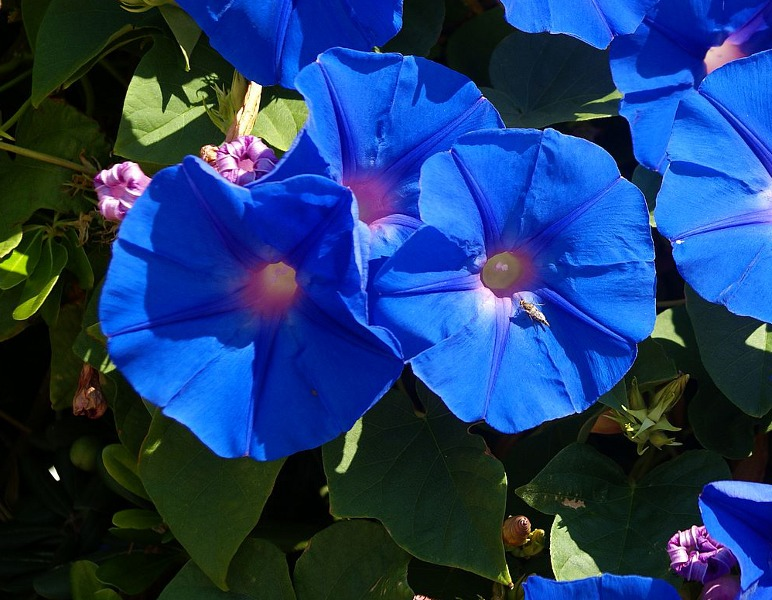
\includegraphics[width=2.5in]{images/segmentation/flowers.jpg}}
%   \end{minipage}% 
%   \begin{minipage}[t]{0.5\linewidth} 
%     \centering 
%     \subfloat[the ROI]{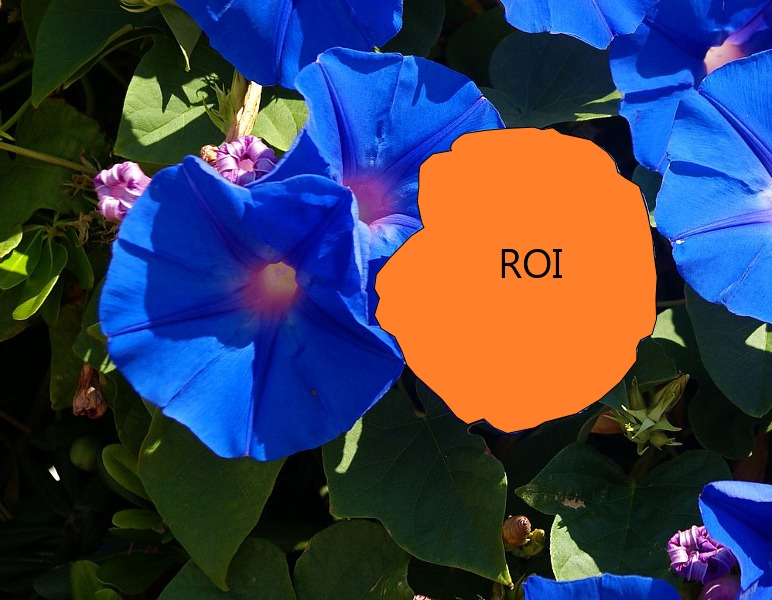
\includegraphics[width=2.5in]{images/segmentation/flowers_m.jpg}}
%   \end{minipage}
% \caption[Segmentation a flower petal from a cluster of flowers]{The
%   origin image is a little clutter, the border of the ROI in b) can
%   not be completely distinguished from the background due poor
%   contrast and shading.}
% \label{fig:flower_m}
% \end{figure}

There are many practical
applications of image segmentation, such as medical imaging, object
tracking, face recognition, fingerprint recognition, machine vision and
so on. In this thesis, we are concerned with object tracking mainly.
In many cases segmentation is the bottleneck when trying to track an
object. Many segmentation methods have been developed, however, there is not
general solution to the segmentation problem. In the real world,
segmentation problems will often require much domain knowledge before
a successful segmentation can be performed. The CCD algorithm is a
powerful method which is combined with the prior knowledge. By
converting a pure segmentation problem to a problem from pattern
recognition field, a large amount of techniques in the field of pattern
recognition are introduced to solve segmentation problems, which are
proved to be effective and helpful. Compared with other segmentation
methods (Fig.~\ref{fig:seg_comparison}), such as intensive-based method,  cluster method, region-based
method and compression-based methods, the CCD algorithm has following
advantages:
\begin{figure}[htbp] 
  \begin{minipage}[t]{0.5\linewidth} 
    \centering 
    \subfloat[Sobel]{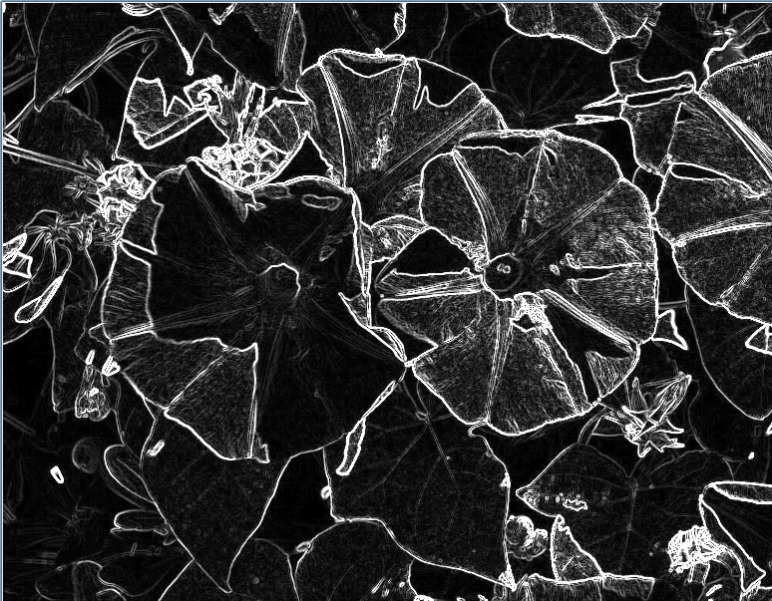
\includegraphics[width=2.5in]{images/flowers_sobel.jpg}}
  \end{minipage} 
  \begin{minipage}[t]{0.5\linewidth} 
    \centering 
    \subfloat[Watershed algorithm]{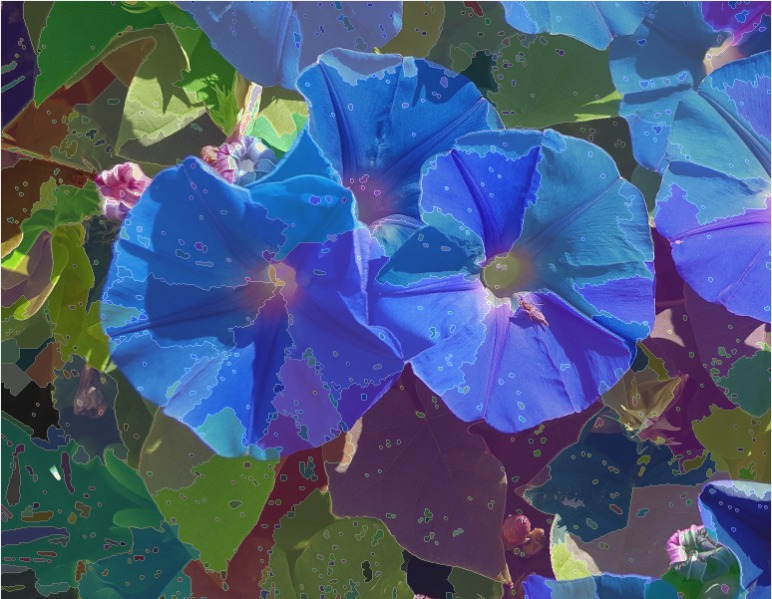
\includegraphics[width=2.5in]{images/flowers_watershed.jpg}}
  \end{minipage} 
  \begin{minipage}[t]{0.5\linewidth} 
    \centering 
    \subfloat[Graph cut]{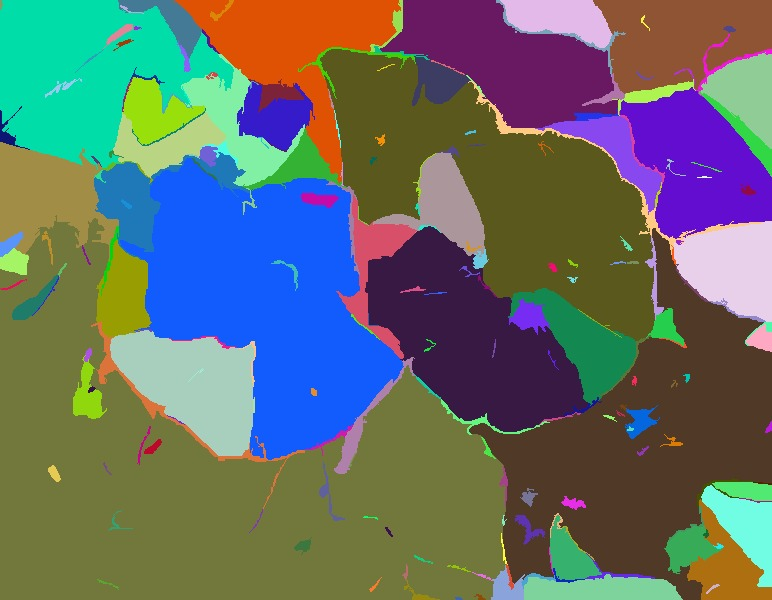
\includegraphics[width=2.5in]{images/flowers_graph.jpg}}
  \end{minipage} 
  \begin{minipage}[t]{0.5\linewidth} 
    \centering 
    \subfloat[Kmeans++]{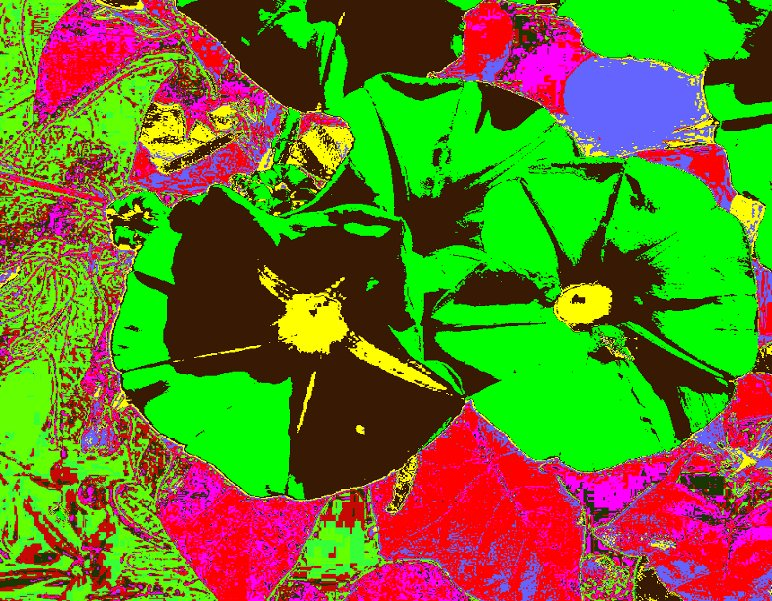
\includegraphics[width=2.5in]{images/flowers_kmeans.jpg}}
  \end{minipage} 
  \begin{minipage}[t]{0.5\linewidth} 
    \centering 
    \subfloat[Expectation and Maximization]{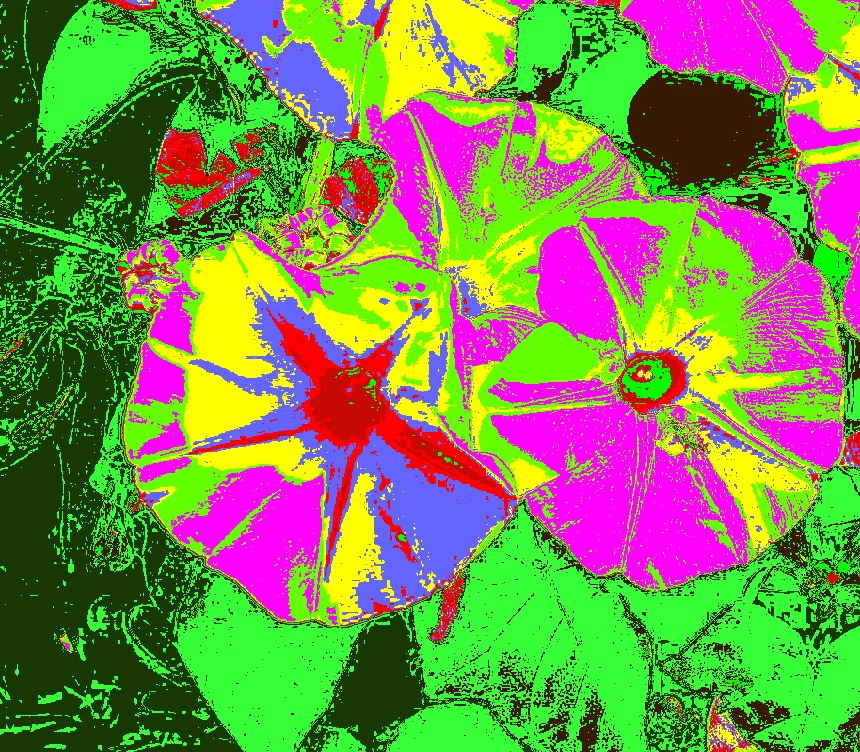
\includegraphics[width=2.5in]{images/flowers_em.jpg}}
  \end{minipage}
  \begin{minipage}[t]{0.5\linewidth} 
    \centering 
    \subfloat[CCD]{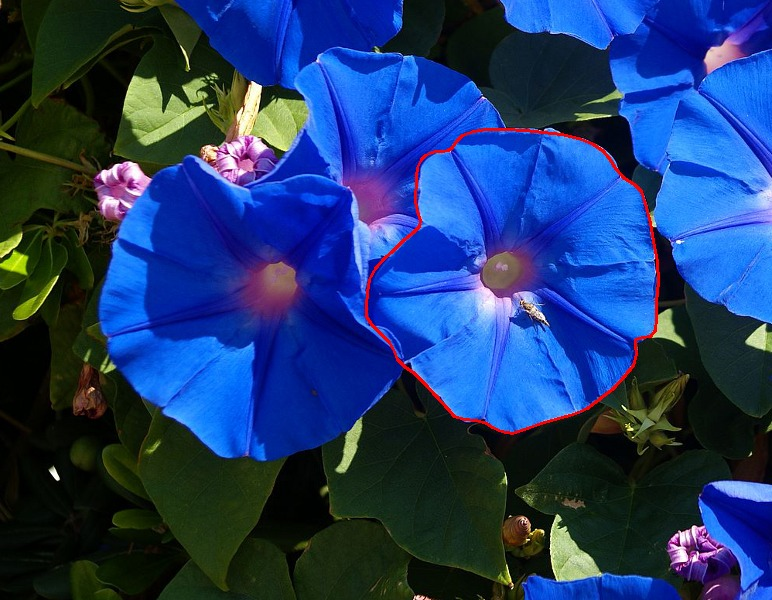
\includegraphics[width=2.5in]{images/flowers_ccd.jpg}}
  \end{minipage}% 
\caption[Resulting images after applying some segmentation methods]{a)
  Edges are detected by a gradient-based algorithm~\cite{scharr2000optimal}. b) Watershed algorithm takes an image as a
  topographic relief. c) Segmentation of an image by defining a predicate for
  measuring the evidence for a boundary between two regions using a
  graph-based representation of the
  image~\cite{felzenszwalb2004efficient}. d) K-means++ algorithm is a
  cluster-based segmentation algorithm~\cite{arthur2007k}. e)
  Segmentation result of Expectation-Maximization (EM) algorithm,
  usually it is initialized by K-means algorithm~\cite{bishop2006pattern}. f) the contour segmented by the CCD
  algorithm discussed in this thesis.}
\label{fig:seg_comparison}
\end{figure}

\begin{itemize}
\item restrict segmentation problem to a limited explicit region: it is helpful
  to decrease the computation cost;
\item probabilistic representation of the variation of the registered
  samples could be easily given, thus statistical inference between
  the model and the image will be applied. All these are helpful to
  improve the segmentation results;
\item the CCD algorithm achieves sub-pixel accuracy and high
  robustness because only a relatively small fraction of the pixels is
  taken into account in the end of iteration.
\end{itemize}

In the following, we apply the proposed CCD algorithm to 4 kind of
objects:
\begin{enumerate}
\item segmentation of a spherical object;
\item segmentation of a 3D object;
\item segmentation of a transparent object;
\item fitting a rigid wire frame.
\end{enumerate}

\subsection{Segmentation of a Ball}
\label{sec:sb}
Like other contour-based methods, we model a contour of the ball as the
prior knowledge. Because the contour for a rigid spherical object is a
circle, besides manually initialization, we can use built-in function in
OpenCV library to generate the contour with given center and
radius. According to the definition of prior distribution, it is required
that the hypothesis is in the range of the variation of
registered samples, namely, the initial contour can not be too far away
from the observed object.

\begin{figure}[htbp] 
  \begin{minipage}[t]{0.5\linewidth} 
    \centering 
        \subfloat[iteration 1]{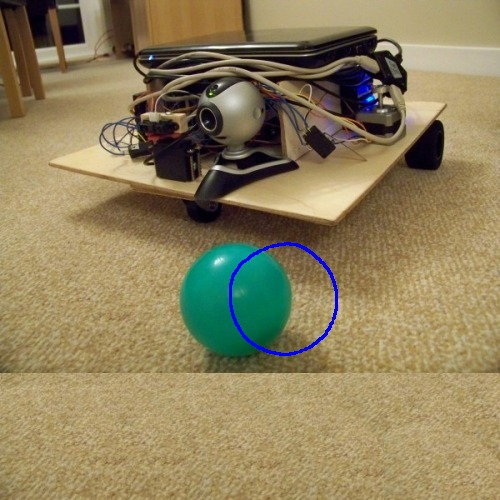
\includegraphics[width=2.5in]{images/ball/0.jpg}}
  \end{minipage}% 
  \begin{minipage}[t]{0.5\linewidth} 
    \centering 
    \subfloat[iteration 3]{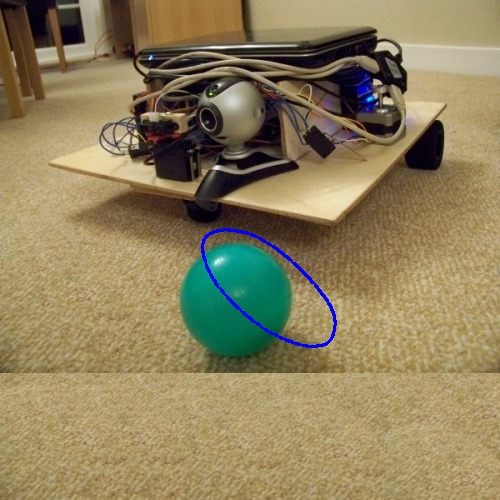
\includegraphics[width=2.5in]{images/ball/2.jpg}}
  \end{minipage} 
  \begin{minipage}[t]{0.5\linewidth} 
    \centering 
    \subfloat[iteration 7]{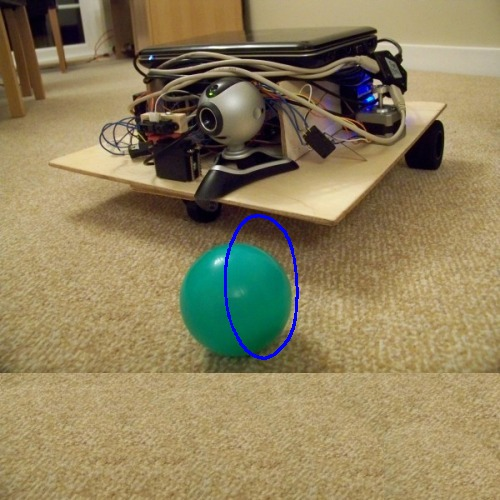
\includegraphics[width=2.5in]{images/ball/6.jpg}}
  \end{minipage} 
  \begin{minipage}[t]{0.5\linewidth} 
    \centering 
    \subfloat[iteration 16]{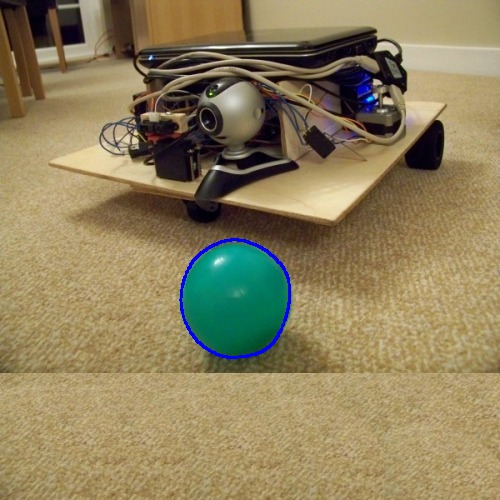
\includegraphics[width=2.5in]{images/ball/15.jpg}}
  \end{minipage} 
\caption[Segmentation of a ball] {a) Rough initialization with the
  mandatory condition that the curve encompasses at least the part of
  the object. b, c) In the beginning, the uncertainty of
  the contour is very large, so the contour is always changing in
  affine-space. After several iterations, it starts to converge and, 
  d) successfully snaps to the obejct.
\label{fig:sab}
}
\end{figure}

In Fig.~\ref{fig:sab}, we intentionally set a hypothesis which is far away
from the ball, but after about 15 iterations, we successfully fit the
contour of the ball. % For the sake of a ground truth we need
% to investigate the pixels used in the iterations. 
Fig.~\ref{fig:pon} shows
that only a small number of pixels are taken into account after the
contour starts to converge but these pixels contain all the
necessary information for refinement of the fitting. Because the
number of sample points used to compute local statistics 
becomes less and less, only a small number of pixels near the boundary
are considered. This makes the CCD algorithm achieve high
sub-pixel accuracy.

\begin{figure}[htbp] 
  \begin{minipage}[t]{0.5\linewidth} 
    \centering 
    \subfloat[iteration 1]{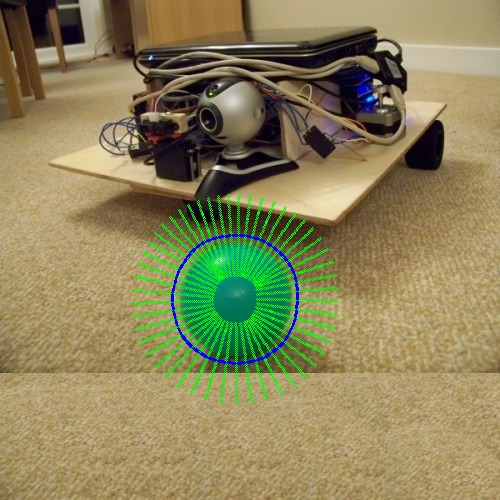
\includegraphics[width=2.5in]{images/ball_normal/0.jpg}}
  \end{minipage}% 
  \begin{minipage}[t]{0.5\linewidth} 
    \centering 
    \subfloat[iteration 3]{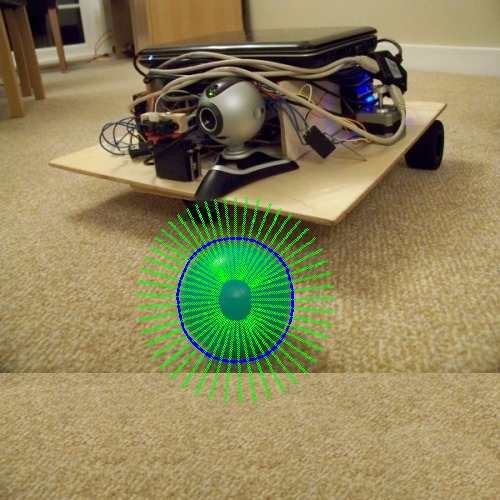
\includegraphics[width=2.5in]{images/ball_normal/1.jpg}}
  \end{minipage} 
  \begin{minipage}[t]{0.5\linewidth} 
    \centering 
    \subfloat[iteration 5]{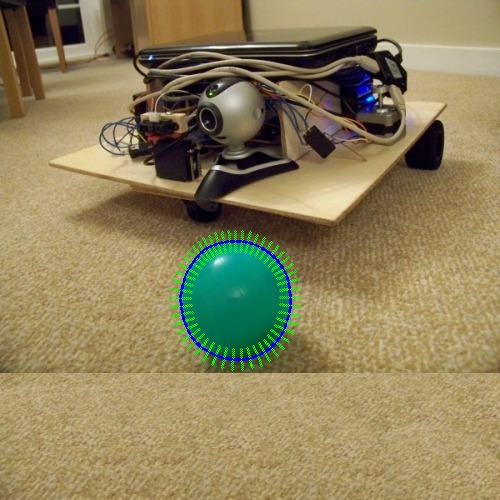
\includegraphics[width=2.5in]{images/ball_normal/3.jpg}}
  \end{minipage} 
  \begin{minipage}[t]{0.5\linewidth} 
    \centering 
    \subfloat[iteration 6]{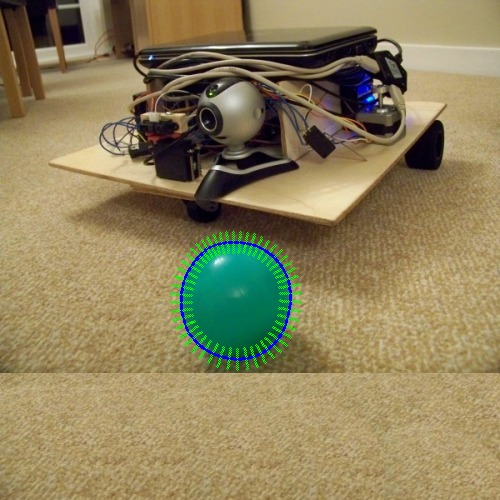
\includegraphics[width=2.5in]{images/ball_normal/4.jpg}}
  \end{minipage} 
\caption[Pixels used in each iteration]{Only a small number of pixels are taken into account after the
contour starts to converge but these pixels contain all the
necessary information for refinement of the fitting. Because the
number of sample points used to compute local statistics 
becomes less and less, only a small number of pixels near the boundary
are considered. This makes the CCD algorithm achieve high
sub-pixel accuracy.}
\label{fig:pon}
\end{figure}


\subsection{Segmentation of a Cuboid-shaped Object}
\label{sec:s3o}
In the experiments of segmenting a spherical object, a planar
affine space of contour is generated. It works very well because the
contour of the ball is always a circle, there is no parallax effect
for such objects. In this case, a 6-dimensional model parameter vector
can cope with basic geometrical transformation of an object. However,
clearly a 6-dimension model parameters vector can not
suffice for non-planar surfaces. Imagine a scenario where we generate the  planar affine
space contour of a non-planar cube in the first view (Fig.~\ref{fig:box_mismatch}a). In the
subsequent view the cube does not lie in the old
space. Due to the parallax effect the mismatch in the fitted contour
will be detected. This is demonstrated in the fitting experiment (Fig.~\ref{fig:box_mismatch}).
\begin{figure}[htbp]
  \begin{minipage}[t]{0.5\linewidth} 
    \centering 
    \subfloat[]{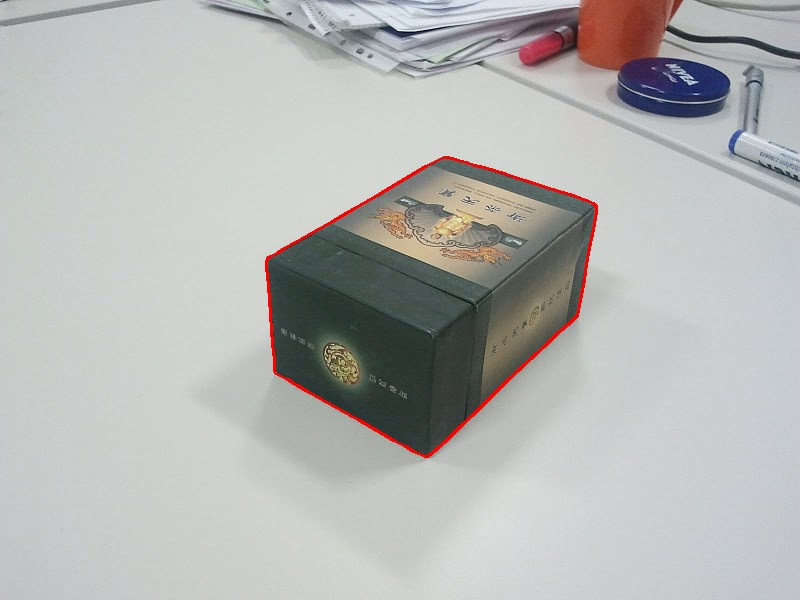
\includegraphics[width=2.5in]{images/box1.jpg}}
  \end{minipage}% 
  \begin{minipage}[t]{0.5\linewidth} 
    \centering 
    \subfloat[]{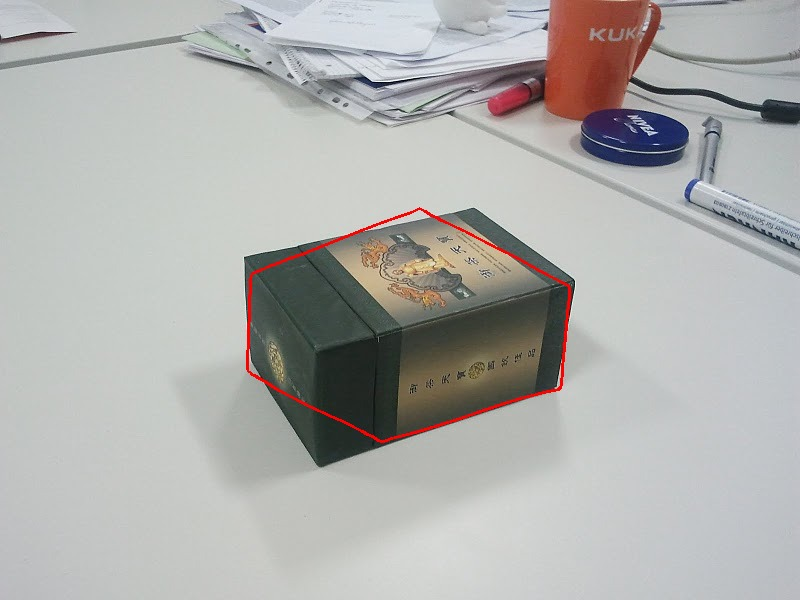
\includegraphics[width=2.5in]{images/box2_mismatch.jpg}}
  \end{minipage} 
  \caption[Planar space can not encompass a general non-planar
  contour]{a) A planar affine space of contours has been fitted from
    the outline of the first view of the cuboid. b) As the viewpoint
    is changed, the outline of the cuboid in the subsequent view does
    not lie in the affine space, which causes visible mismatch in the
    fitted contours.}
\label{fig:box_mismatch}
\end{figure}


% The new 3D affine shape-space with 8 degree of freedom,
% made up of the 6-parameter planar affine space and a two-parameter
% extension, is designed to cope with such problem. 
In order to account for this issue we introduced the 3D affine
shape-space with 8 DOFs.
Two added components
account for the depth variation that is not visible in the template
view. After adding the two new parameters to the shape matrix, the form
of shape matrix for 3D case can be given as follows:
\begin{equation}
  \label{eq:4.18}
  A =
  \begin{bmatrix}
    1 & 0 & P_0^x & 0 & 0 & P_0^y & P_0^z & 0\\
    0 & 1 & 0 & P_0^y & P_0^x & 0 & 0  & P_0^z
  \end{bmatrix}\qquad.
\end{equation}

\begin{figure}[htbp]
  \begin{minipage}[t]{0.5\linewidth} 
    \centering 
    \subfloat[]{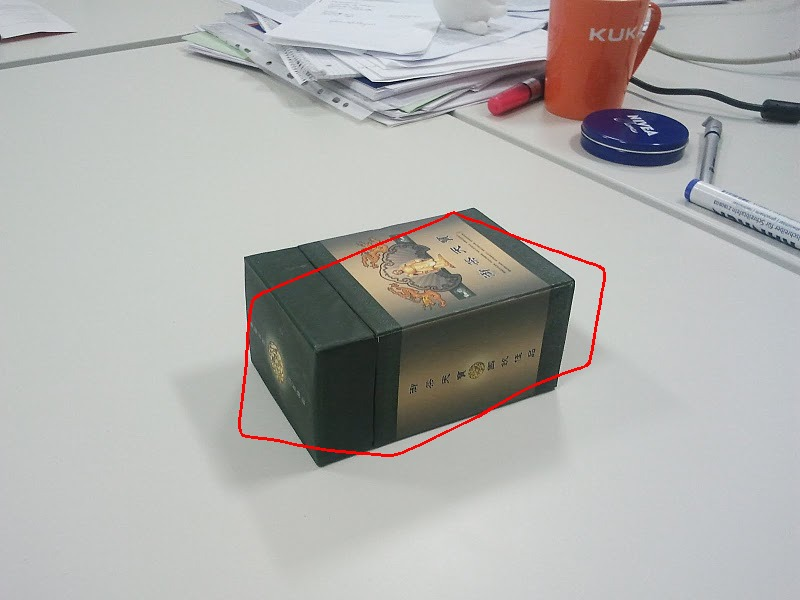
\includegraphics[width=2.5in]{images/box2_3d.jpg}}
  \end{minipage}% 
  \begin{minipage}[t]{0.5\linewidth} 
    \centering 
    \subfloat[]{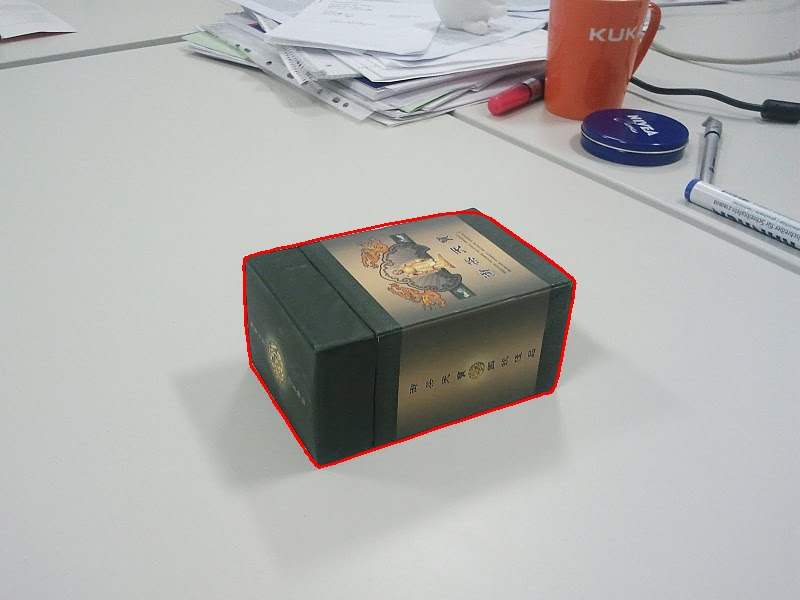
\includegraphics[width=2.5in]{images/box2_ok.jpg}}
  \end{minipage} 
  \caption[Fitting the contour of non-planar object]{Using 3D
    affine shape-space fitting of a contour to the non-planar object
    becomes possible.}
\label{fig:box_match}
\end{figure}

The 3D affine shape-space model parameters have
the following interpretation

\begin{equation}
  \label{eq:4.19}
  \mathbf{\Phi} =  (T_1, T_2, M_{11} - 1, M_{22} - 1, M_{21}, M_{12}, \nu_1, \nu_2)
\end{equation}

The expanded space now encompasses the object in all views as depicted
in Fig.~\ref{fig:box_match}. At last, we do
another experiment for an object with an irregular shape (Fig.~\ref{fig:container}). This
demonstrates that the CCD works well for 3D non-planar object, too.

\begin{figure}[htbp] 
  \begin{minipage}[t]{0.5\linewidth} 
    \centering 
    \subfloat[iteration 1]{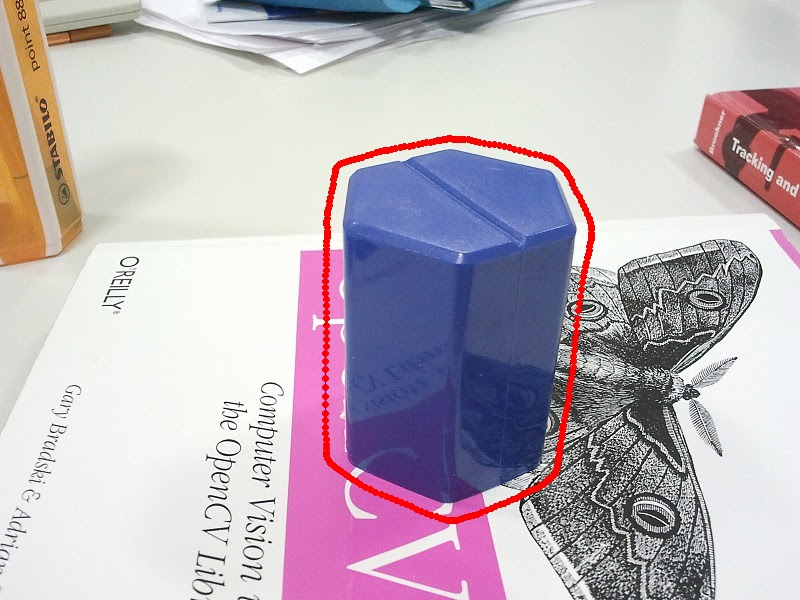
\includegraphics[width=2.5in]{images/container/0.jpg}}
  \end{minipage}% 
  \begin{minipage}[t]{0.5\linewidth} 
    \centering 
    \subfloat[iteration 2]{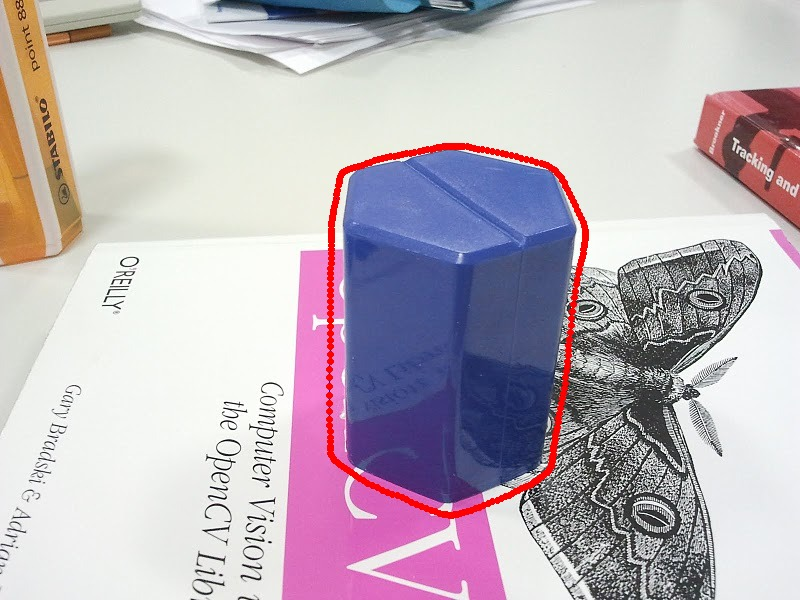
\includegraphics[width=2.5in]{images/container/1.jpg}}
  \end{minipage} 
  \begin{minipage}[t]{0.5\linewidth} 
    \centering 
    \subfloat[iteration 4]{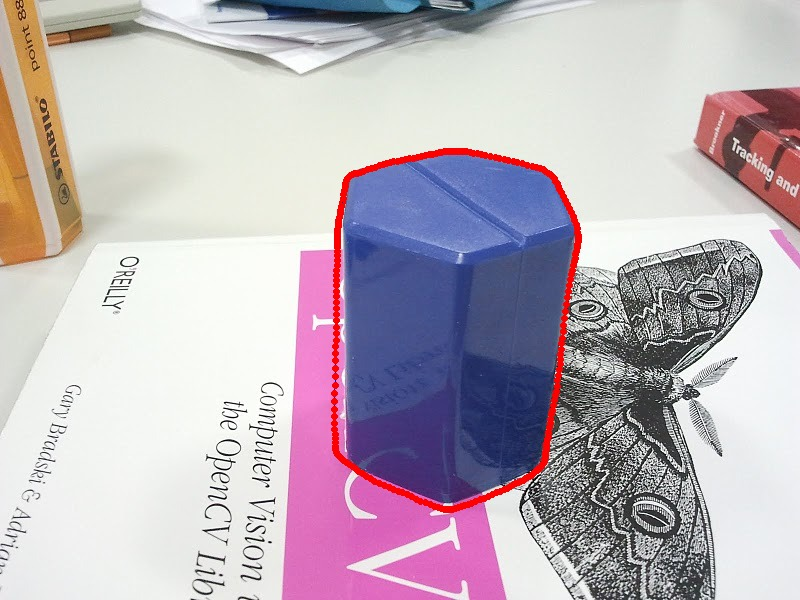
\includegraphics[width=2.5in]{images/container/2.jpg}}
  \end{minipage} 
  \begin{minipage}[t]{0.5\linewidth} 
    \centering 
    \subfloat[iteration 7]{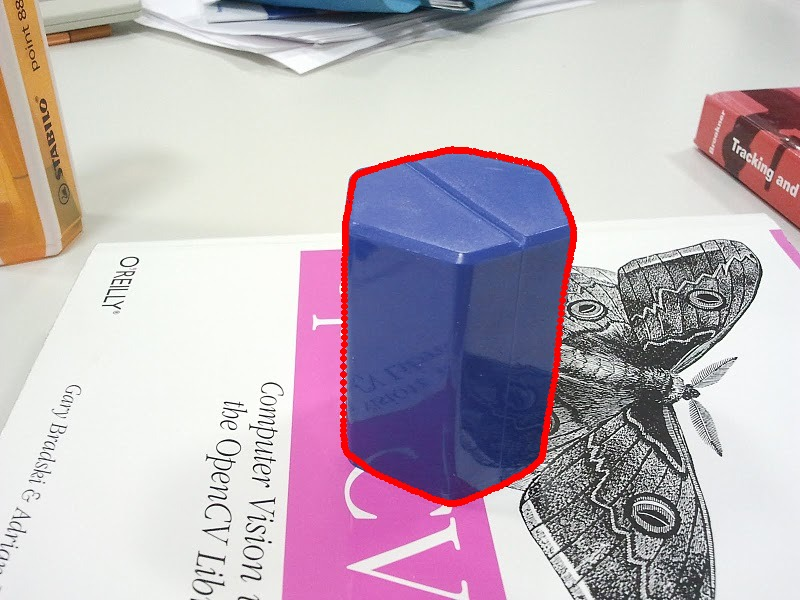
\includegraphics[width=2.5in]{images/container/5.jpg}}
  \end{minipage} 
\caption[3D affine shape-space for rigid object]{The
  non-planar polyhedron is encompassed by a 3D affine space.}
\label{fig:container}
\end{figure}

\subsection{Segmentation of a Transparent Object}
\label{sec:sto}
In this thesis, local statistical information is collected in terms of
pixel intensity in the vicinity of a contour, which leads to a poor
result for transparent objects. In this experiment, the
target is a Cocacola bottle whose upper part is nearly transparent and the
lower part is opaque. The result in Fig.~\ref{fig:cola} shows that the CCD algorithm
segments the lower part but fails to completely encompass the contour in the
upper part. However, because the model only has 6 (or 8
for 3D object) DOFs, the convergence of the lower part will aid the convergence for the whole object.


\begin{figure}[htbp] 
  \begin{minipage}[t]{0.5\linewidth} 
    \centering 
    \subfloat[iteration 1]{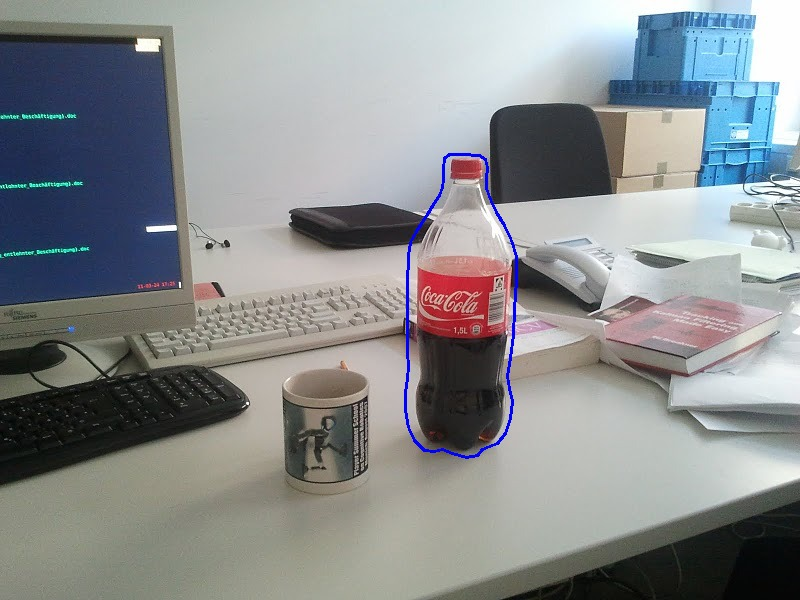
\includegraphics[width=2.5in]{images/bottle/0.jpg}}
  \end{minipage}% 
  \begin{minipage}[t]{0.5\linewidth} 
    \centering 
    \subfloat[iteration 2]{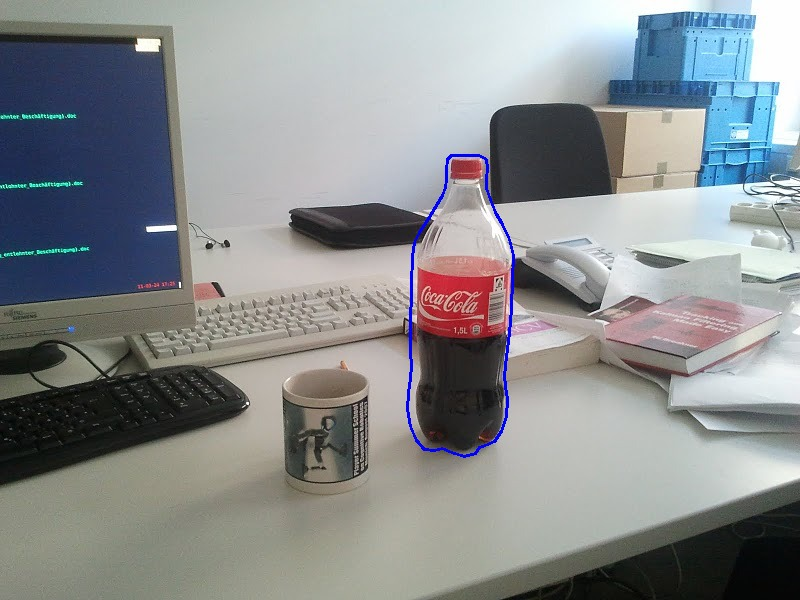
\includegraphics[width=2.5in]{images/bottle/1.jpg}}
  \end{minipage} 
  \begin{minipage}[t]{0.5\linewidth} 
    \centering 
    \subfloat[iteration 3]{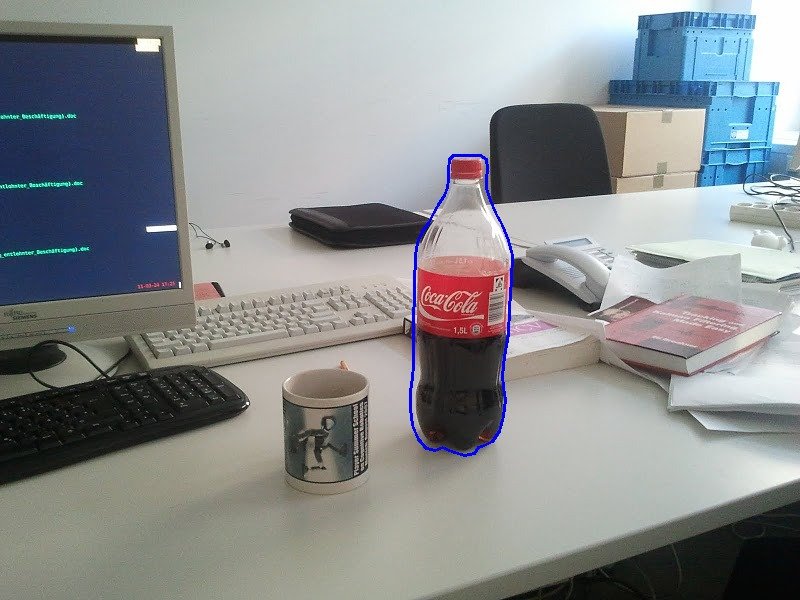
\includegraphics[width=2.5in]{images/bottle/2.jpg}}
  \end{minipage} 
  \begin{minipage}[t]{0.5\linewidth} 
    \centering 
    \subfloat[iteration 21]{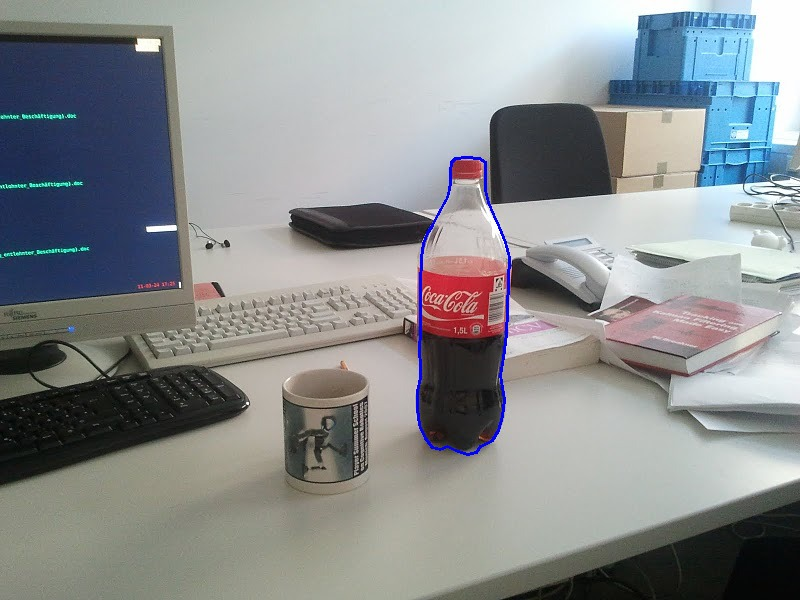
\includegraphics[width=2.5in]{images/bottle/20.jpg}}
  \end{minipage} 
\caption[An example of a successful convergence for the half-transparent object]{An example of a
  successful convergence for the half-transparent object. In image (d), due to the shadow and poor
contrast, the contour does not completely attach to the edge of the
bottom. Moreover, in the transparent part of the bottle, the outline
closely attaches to the edge in the left but stays away from the edge
in the right. The transparency leads to the difficulties. }
\label{fig:cola}
\end{figure}


% \subsection{Fitting a Rigid Wire Frame}
% \label{sec:fdo}
% In the following, we fit a rigid wire frame model to the image
% depicted in Fig.~\ref{fig:wireframe}.  The degrees of freedom
% are the 8 pose parameters. This experiment demonstrates that the CCD
% algorithm is not only able to exploit object contours, but it can also
% use internal model edges separating multiple, possibly dependent,
% image regions.  The CCD algorithm reliably estimates the pose of the box despite
% the partial occlusion.

% \begin{figure}[htbp] 
%   \begin{minipage}[t]{0.5\linewidth} 
%     \centering  
%     \subfloat[iteration 1]{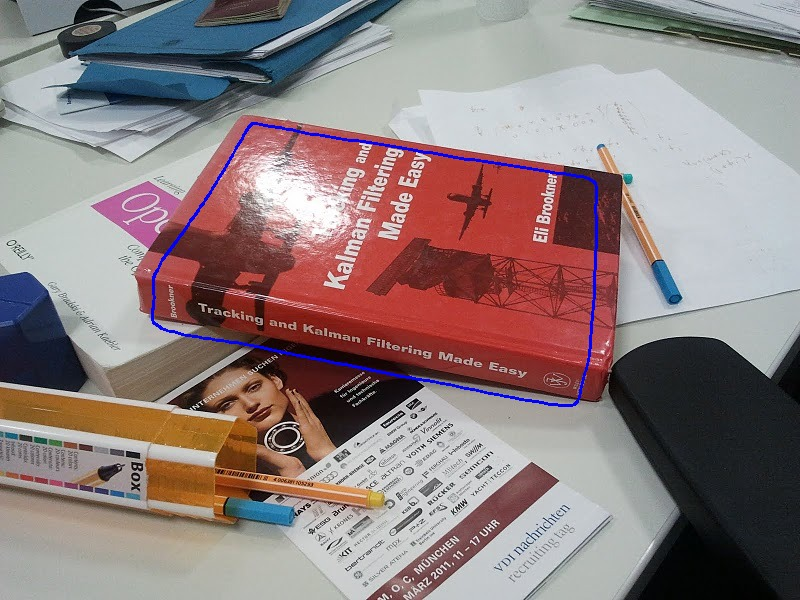
\includegraphics[width=2.5in]{images/book/0.jpg}}    
%   \end{minipage}% 
%   \begin{minipage}[t]{0.5\linewidth} 
%     \centering 
%     \subfloat[iteration 2]{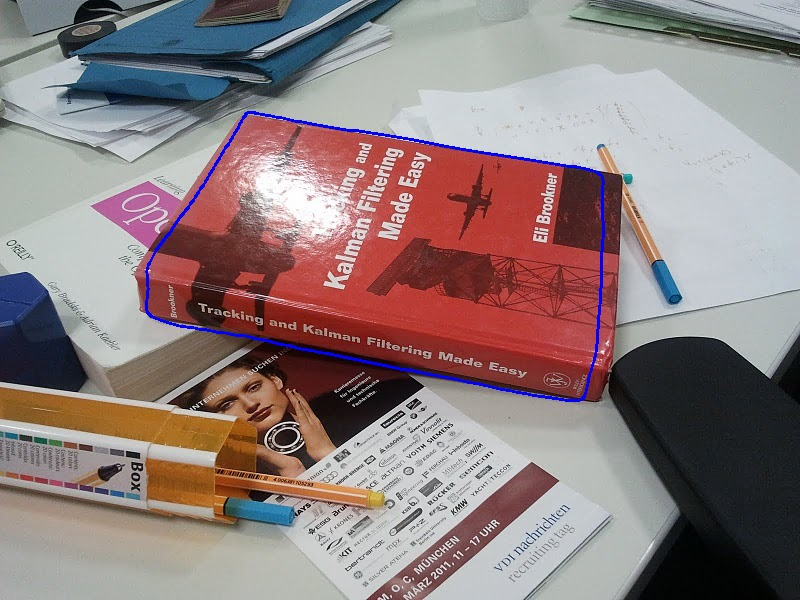
\includegraphics[width=2.5in]{images/book/1.jpg}}
%   \end{minipage} 
%   \begin{minipage}[t]{0.5\linewidth} 
%     \centering 
%     \subfloat[iteration 3]{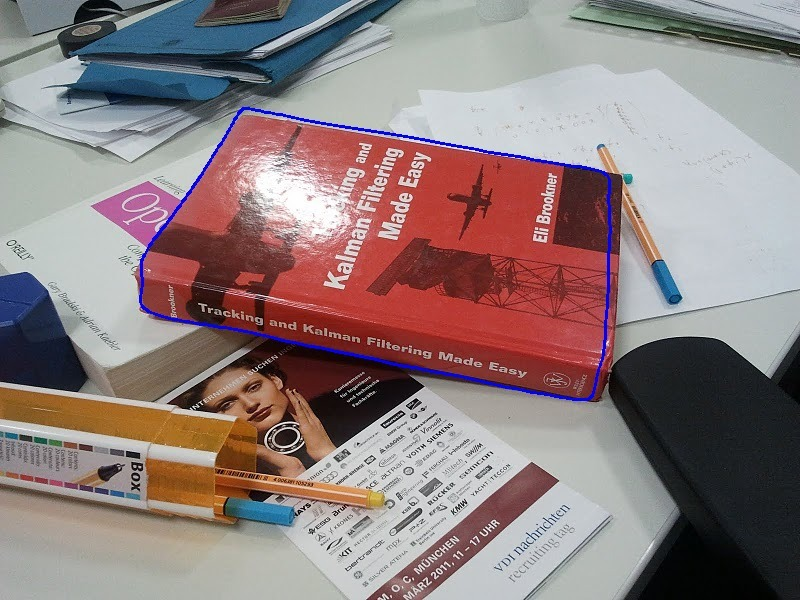
\includegraphics[width=2.5in]{images/book/2.jpg}}
%     \label{subfig:iteration 3}
%   \end{minipage} 
%   \begin{minipage}[t]{0.5\linewidth} 
%     \centering 
%     \subfloat[iteration 14]{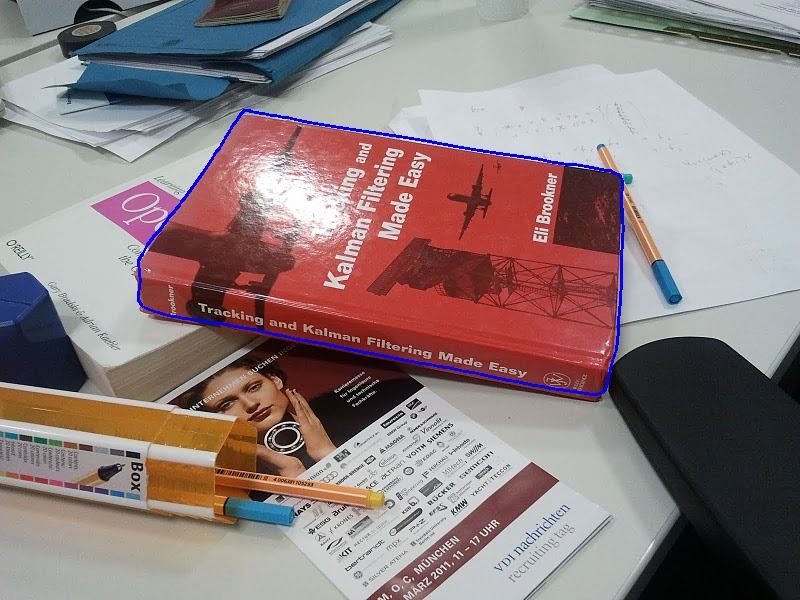
\includegraphics[width=2.5in]{images/book/13.jpg}}
%   \end{minipage}
%   \begin{minipage}[t]{\linewidth} 
%     \centering 
%     \subfloat[segmentation of edge-based algorithm]{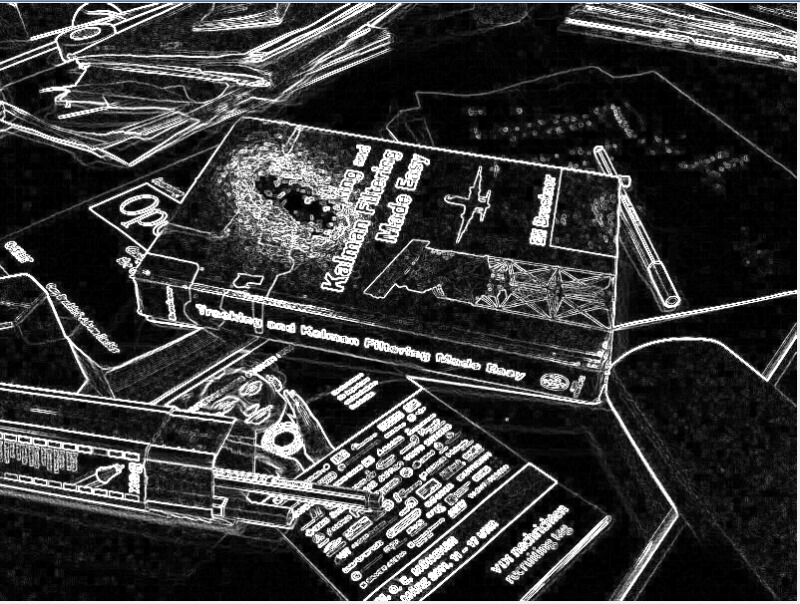
\includegraphics[width=0.8\linewidth]{images/book/book_sobel.jpg}}
%   \end{minipage} 
% \caption[Fitting a rigid wire frame in a inhomogeneous background]{The book
%   is located in a partially occluded background. From (a)-(d), despite
% the variation of the illumination and contrast, the CCD algorithm
% accurately fits a wire frame model to the image data. In (e), here the
% edge-based algorithm yields some errors.}
% \label{fig:wireframe}
% \end{figure}


\section{Track Initialization from SIFT Features}
\label{sec:sift_init}
Scale-invariant feature transform (or SIFT) is an algorithm to detect
and describe local features in images.  It is widely used to solve
many problems in the field of Computer Vision, such as object
recognition, robotic mapping and navigation, and video tracking. There are four key stages in the sift algorithm~\cite{lowe2004distinctive}:
\begin{enumerate}
\item \textbf{Scale-invariant feature detection}: an image is transformed into
  a collection of vectors which are scale-invariant. By applying a Difference-of-Gaussian
function to a series of smoothed and resampled images, potential
interest points are identified.
\item \textbf{Keypoint localization and indexing}: keypoints are selected at given
  candidate location, and then stored as SIFT keys.
\item \textbf{Orientation assignment}:  one or more orientations are assigned to each keypoint lo-
cation based on local image gradient directions. All future operations are performed
on image data that has been transformed relative to the assigned orientation, scale, and
location for each feature, thereby providing invariance to these transformations.
\item \textbf{Keypoint descriptor}: the local image gradients are measured at the selected scale
in the region around each keypoint. These are transformed into a representation that
allows for significant levels of local shape distortion and change in illumination.
\end{enumerate}


The SIFT keypoints and features are local and based on the appearance
of the object at particular interest points. The SIFT algorithm has following
features and advantages:
\begin{itemize}
\item Invariant to image scale and rotation, robust to changes in
  illumination and minor changes in viewpoint.
\item Highly distinctive, easy to extract, allow for correct object
  identification and easy to match against a database of local
  features. 
\item Need few features (as few as 3) from an object to compute its location
  and pose. Computation cost is moderate on modern computer hardware.
\end{itemize}

% Based on these features, SIFT is usable for object recognition, the
% steps are given below.
% \begin{itemize}
% \item Extract SIFT features from a series of input template image,
%   then store these features into a database.
% \item Given a new input image, after training, the features in
%   the image are matched to the SIFT feature database obtained from the
%   training images.
% \end{itemize}

In this thesis, we use the SIFT algorithm to initialize the
contour of an object. Assume we have marked the boundary points in the
training images. In order to project these boundary points to the test
image, it is essential to estimate the homography between the
images. However, SIFT matching
might lead to lots of "false" matches. % In order
% to evaluate the homography, firstly we have to exclude the
% mismatches. 
For filtering out false positives, we use RANSAC, which is an
iterative process that randomly selects enough matches to fit the
homography. It contains the following steps~\cite{fischler1981random}.

\begin{itemize}
\item  Randomly select a sample of matched points and instantiate the
  model from this subset.
\item Determine the set of data points that are within a distance
  threshold of the homography. The set is the consensus set of the sample
  and defines the inliers.
\item If the size of the set (e.g. the number of inliers) is greater
  than some threshold, re-estimate the homography using all the matched
  points and terminate. Otherwise, select a new subset and repeat the
  above.
\item After some trials the largest consensus set is selected, and the
  homography is re-estimated using all the points in the subset.
\end{itemize}
Fast way to compute the homography in a least squares sense is to use the Normalized
Direct Linear Transform (normalized
DLT)~\cite{hartley2003multiple}. The Normalized DLT algorithm computes
a homography for a projective transformation by using at least 4 point
correspondences and then minimizing corresponding norm.

After obtaining the homography between the template image and the
test image, the contour of object can be easily projected
into the test image to obtain the estimate of the contour
position. This is illustrated in Fig.~\ref{fig:sift} and
Fig.~\ref{fig:sift_result}. Note that because SIFT is only invariant
to minor changes in view points, the method does not always work for
non-planar objects which have substantially different view points.

\begin{figure}[htbp]
  \centering
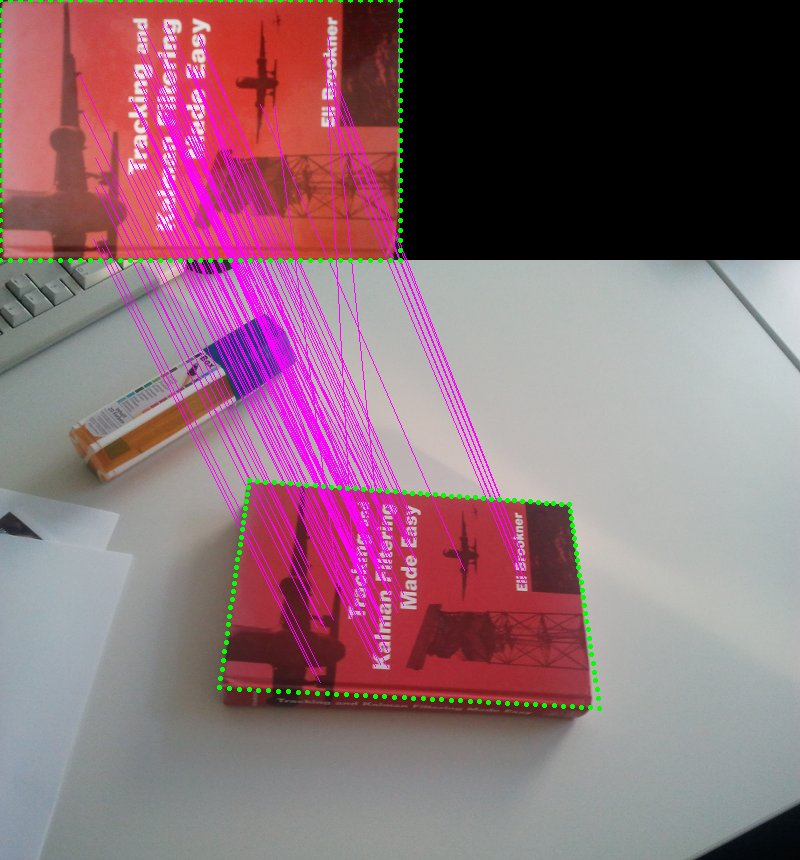
\includegraphics[width=\linewidth]{images/sift.jpg}
\caption[Contour initialization using the SIFT algorithm]{The image in
  the upper-left corner is a template. It is projected into the bottom
  image. The green points in the template image encompass the
  contour of the observed object. The red lines are used to connect the matching feature
  points. Obviously, the outliers are excluded using the RANSAC
  algorithm. The homography is then estimated from these matching
  feature points.  After finding a perspective
  transformation from the matching features, the source contour is
  projected onto the image in the bottom, and used as initial contour
  for the CCD algorithm.}
\label{fig:sift}
\end{figure}

\begin{figure}[htbp]
  \centering
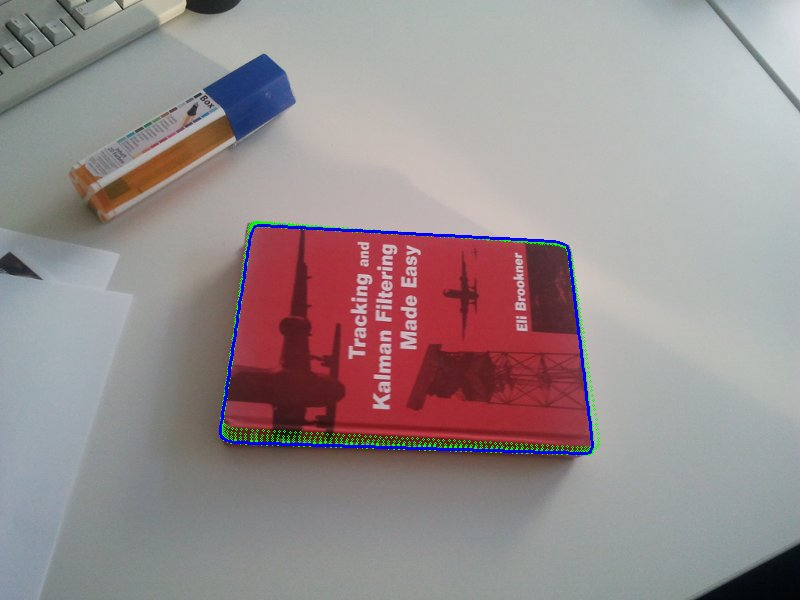
\includegraphics[width=\linewidth]{images/sift_result.jpg}
\caption[The contour obtained using the CCD algorithm converges to the
edge of the book]{After 8 iterations, the contour obtained in Fig.~\ref{fig:sift} converges to the edge of the book.}
\label{fig:sift_result}
\end{figure}

% The model hypothesis is obtained by applying the CCD algorithm to a
% frame of a video sequence. In the following experiments, we can test
% our naive CCD tracker on PR2, the result is demonstrated in Fig.~\ref{fig:sifttracker} 

\begin{figure}[htbp]
  \begin{minipage}[t]{0.5\linewidth} 
    \centering  
    \subfloat[Sampled frame 1]{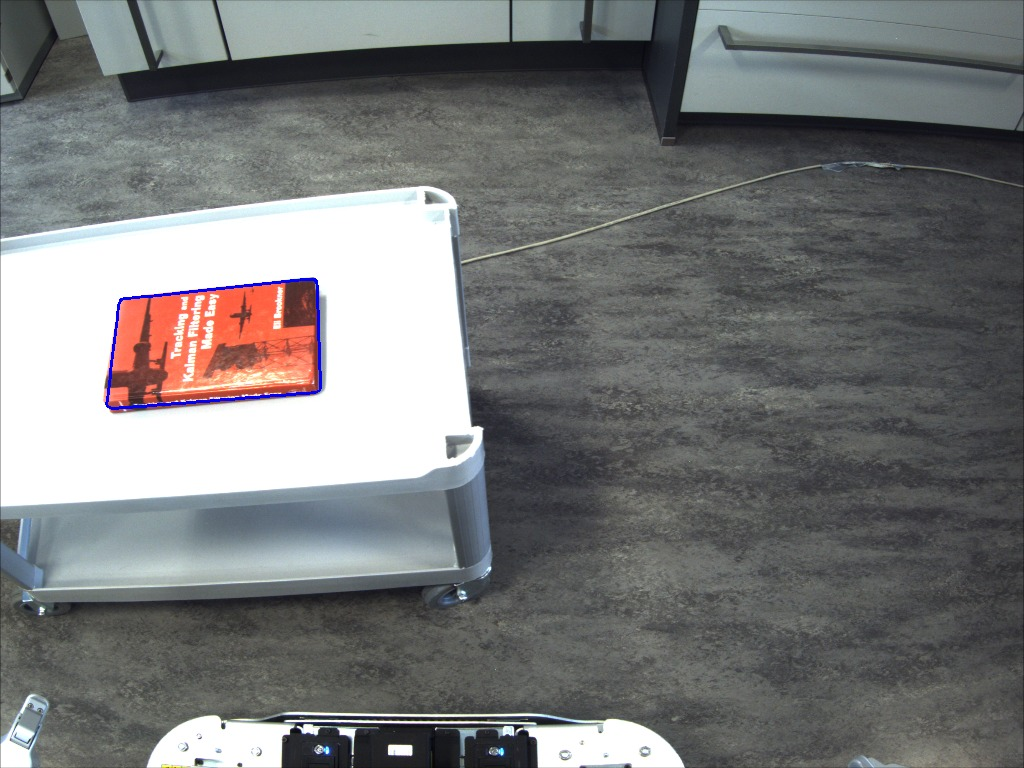
\includegraphics[width=2.5in]{images/sift/1.jpg}}    
  \end{minipage}% 
  \begin{minipage}[t]{0.5\linewidth} 
    \centering 
    \subfloat[Sampled frame 2]{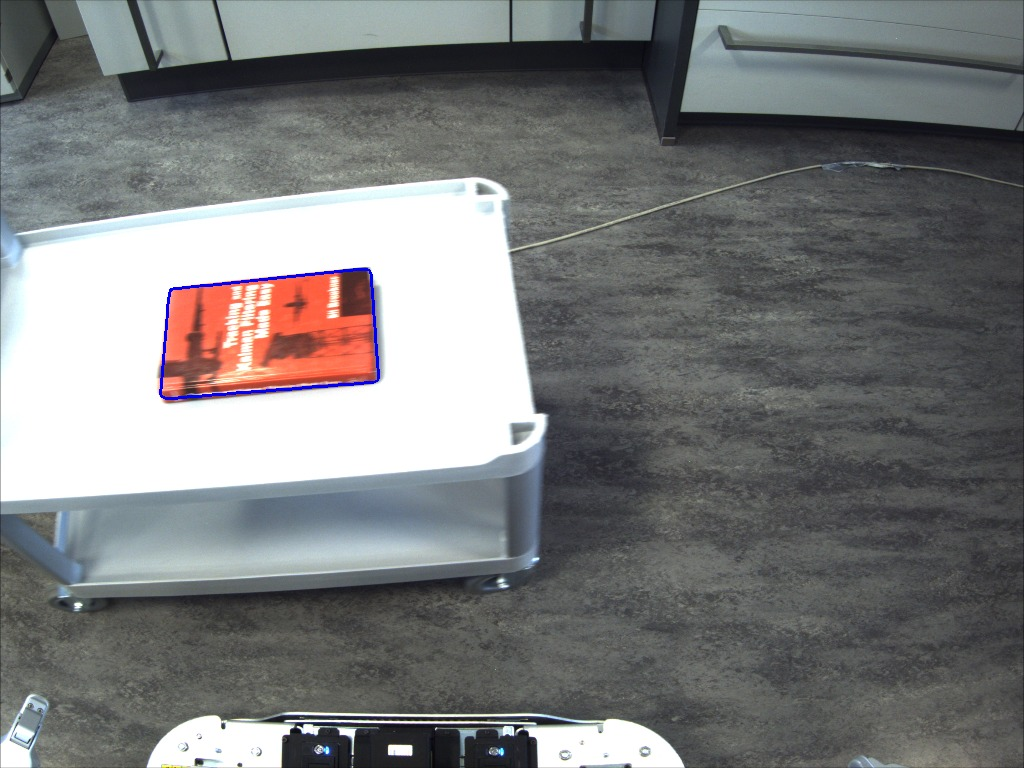
\includegraphics[width=2.5in]{images/sift/10.jpg}}
  \end{minipage} 
  \begin{minipage}[t]{0.5\linewidth} 
    \centering 
    \subfloat[Sampled frame 3]{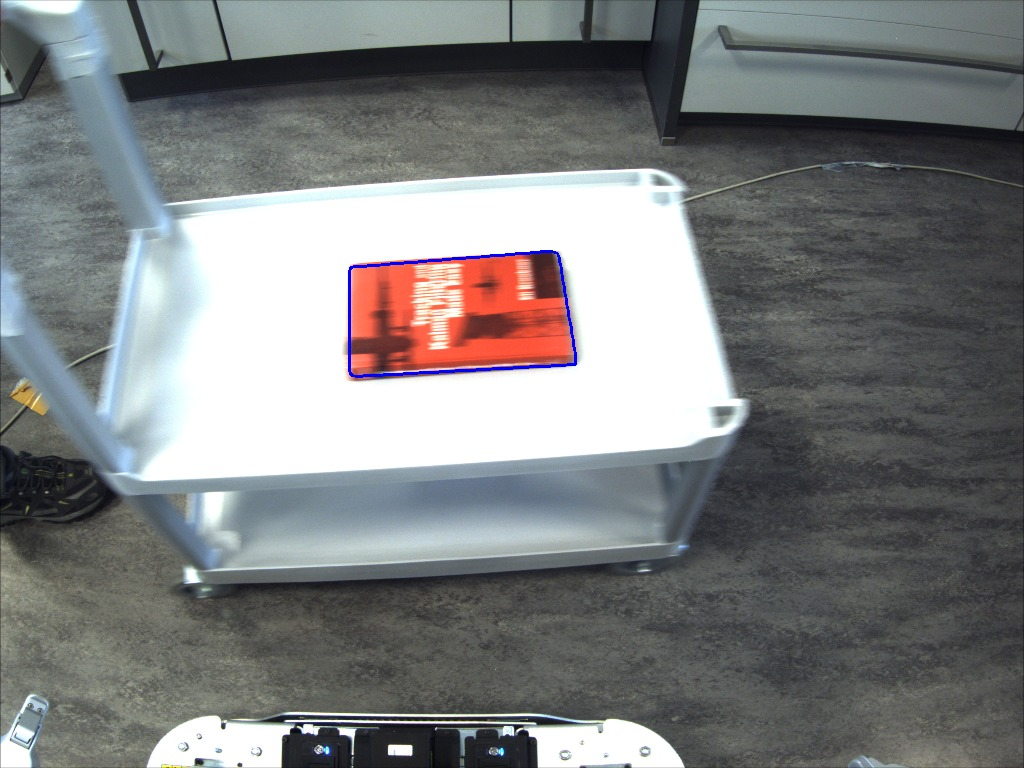
\includegraphics[width=2.5in]{images/sift/30.jpg}}
    \label{subfig:iteration 3}
  \end{minipage} 
  \begin{minipage}[t]{0.5\linewidth} 
    \centering 
    \subfloat[Sampled frame 4]{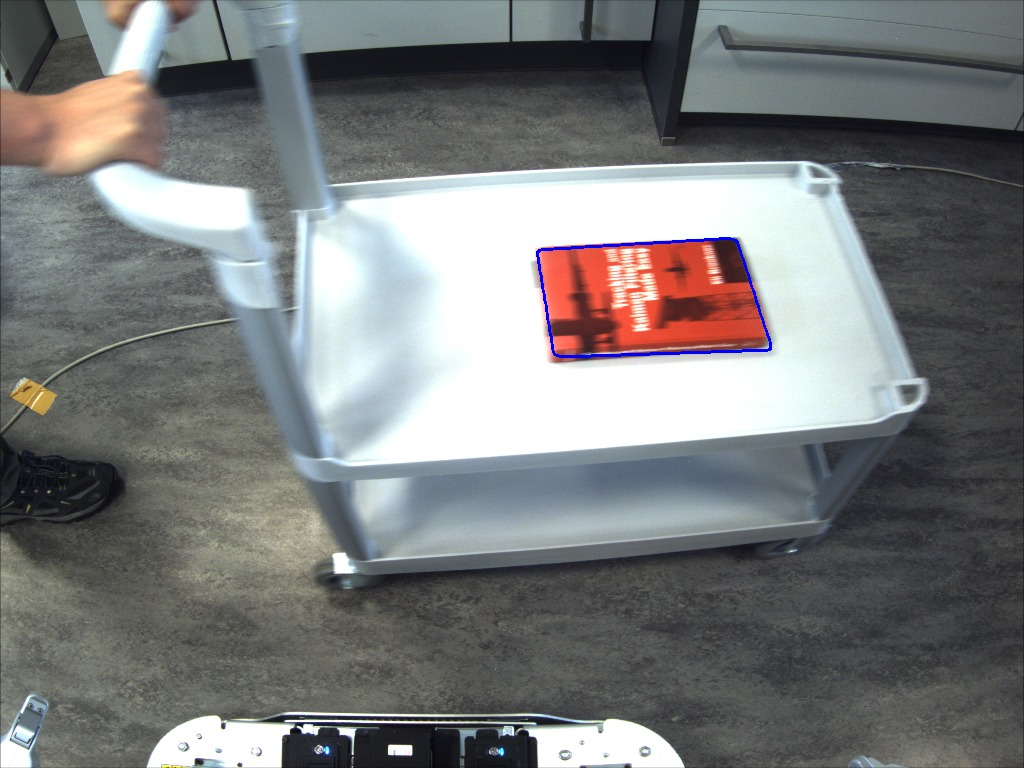
\includegraphics[width=2.5in]{images/sift/45.jpg}}
  \end{minipage} 
  \begin{minipage}[t]{0.5\linewidth} 
    \centering 
    \subfloat[Sampled frame 5]{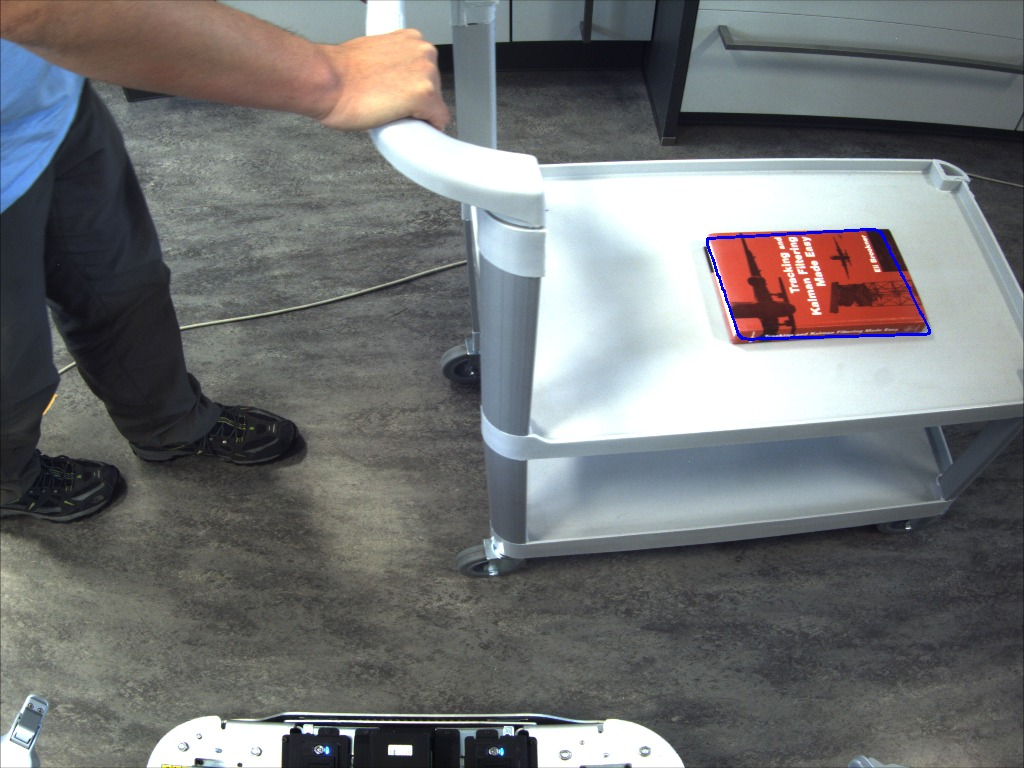
\includegraphics[width=2.5in]{images/sift/63.jpg}}
  \end{minipage} 
  \begin{minipage}[t]{0.5\linewidth} 
    \centering 
    \subfloat[Sampled frame 6]{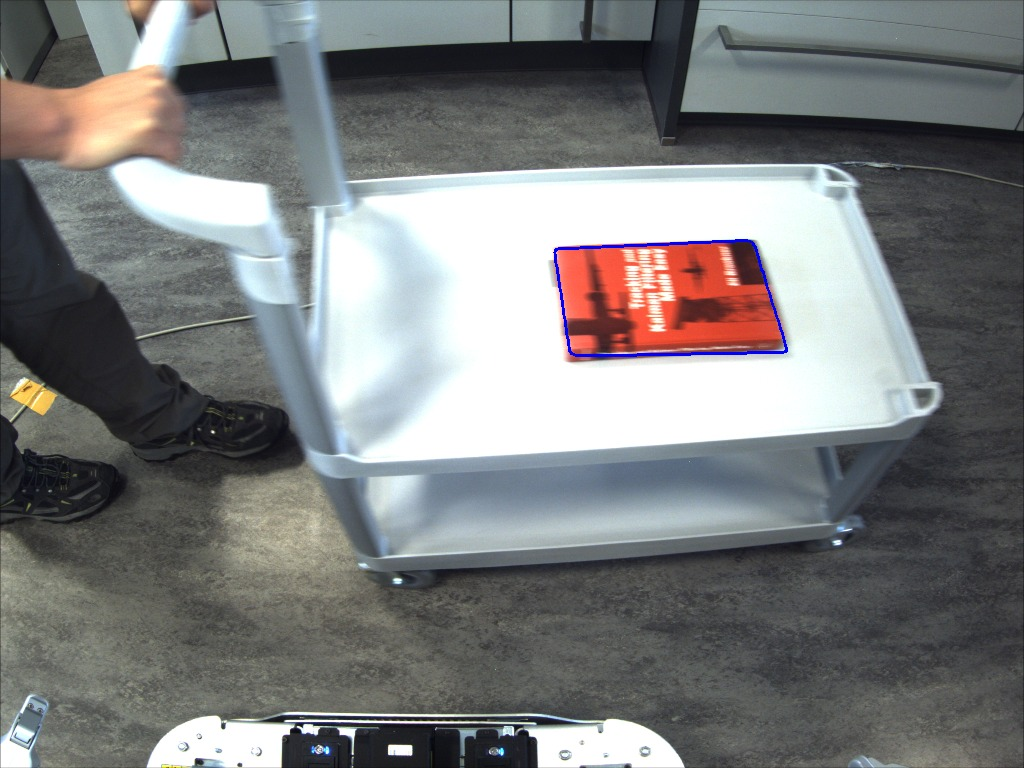
\includegraphics[width=2.5in]{images/sift/80.jpg}}
  \end{minipage} 
  \caption[The tracking result based on SIFT contour initialization]{The
    CCD tracker successfully tracks the motion of a book.
  }
  \label{fig:sifttracker}
\end{figure}


\section{Track Initialization from 3D Point Cloud}
\label{sec:tifpc}

A point cloud is a set of vertices created by 3D
scanners. The scanners measure points on the surface of an object,
therefore, a point cloud represents the set of points measured by the
device. Point clouds cloud are widely used to  create 3D CAD models
for manufactured parts, a multitude of visualization, animation and
rendering.
\begin{figure}[htb]
  \centering
  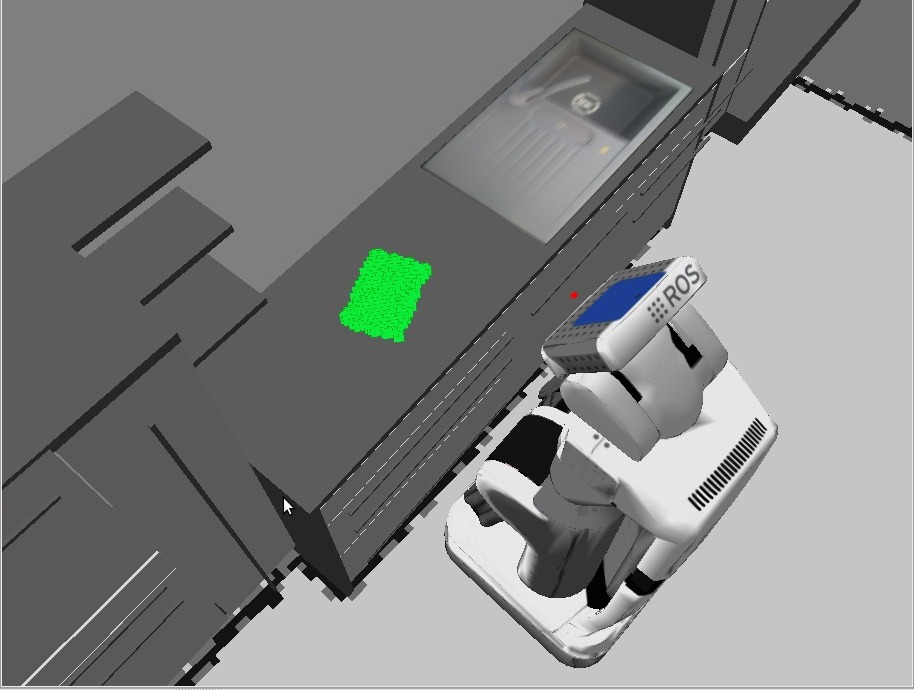
\includegraphics[width=\linewidth]{images/pr2b.jpg}
  \caption[Kinect camera of the PR2 Robot and object candidate
  segmented in 3D point cloud.]{Kinect camera of
    the PR2 Robot and object candidate segmented in 3D point
    cloud. Encompassing a contour of the back-projected points onto
    the image is used as an initial contour for the CCD algorithm.}
  \label{fig:pointcloud}
\end{figure}

Point clouds can be rendered and inspected in software like MeshLab
and rviz (Fig.~\ref{fig:pointcloud}). In addition, they are usually converted to polygon or
triangle mesh models, NURBS surface models, or CAD models through a
process commonly referred to as surface reconstruction.

In this experiments, we plan to convert a point cloud of an object to a
polygon, then use this polygon as the initial contour of observed
object. In the point cloud in Fig.~\ref{fig:pointcloud}, edges of
the observed object are not smoothed. By applying the CCD algorithm,
we can accurately obtain the contour of a observed object. In
comparison with the initialization from SIFT features, because the
outlines created from point cloud is 3D, it is more
suitable for non-planar objects.
